\chapter{Совместное использование сильно и слабо размеченных набооров данных} \label{chapt3}

\section{Мотивация} \label{sect3_1}

Как было сказано в предыдущей главе, классический MIL имеет ряд ограничний в том числе на размер карты. Поэтому были сформулированы следущие задачи:

\begin{itemize}
    \item Создать систему, которая способна возвращать карты сегментации высокого разрешения;
    \item Оснастить данную систему возможностью обучаться как на сильно так и на слабо размеченных наборах данных;
\end{itemize}

При решении даннных задач было обращено внимание на \cite{rongchang_weakly-supervised_2018}, где авторы уже решали подобную задачу. Они предложили пирамидальную интегральную структуру слоёв нейросети, которая один за одним последовательно суммирует с различными коэффициентами значения слоёв сети, с каждым шагом увеличивая размерность. В результате ряда экспериментов, мы остановились на архитектуре, изображенной на рис. \ref{fig:schema_total}. При этом предлагается следующий порядок обучения системы(рис. \ref{fig:schema_order}):

\begin{figure}[h] 
  \center
  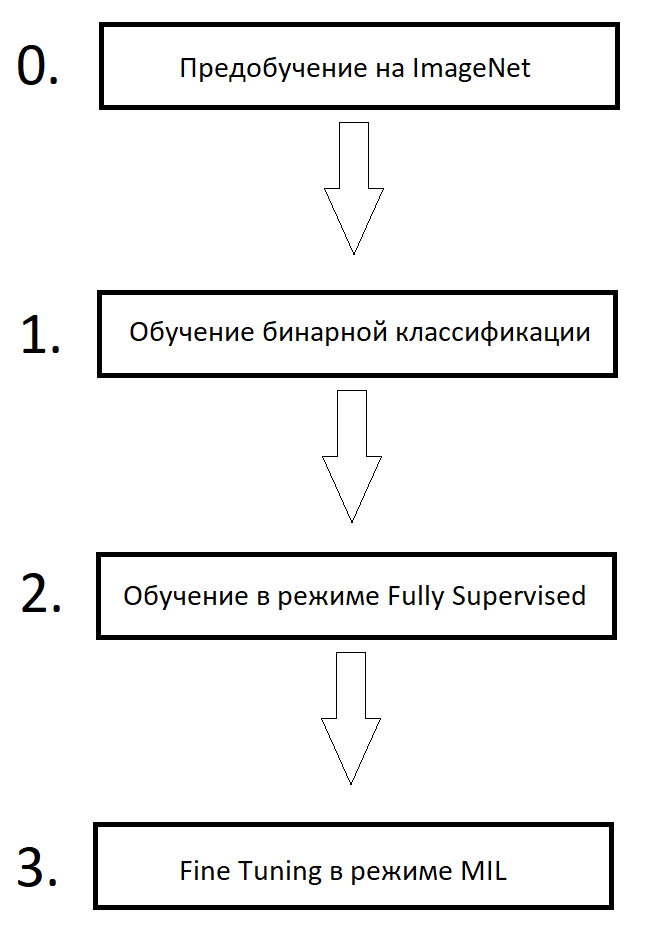
\includegraphics [scale=0.4] {images/schema.png}
  \caption{Порядок обучения} 
  \label{fig:schema_order}  
\end{figure}

Остановимся на каждом из этапов подробнее.

\begin{enumerate}[start=0]
    \item Инициализация весов ResNet-50 весами предобучения на ImageNet позволяет ускорить дообучение геометрических признаков, так как часть геометрических конфигураций уже усвоена сетью;
    \item Данный пункт будет изучен ниже. Выдвигается гипотеза, что, поскольку, распределение данных на ImageNet сильно отличается от распределения медицинских изображений, то имеет смысл сперва обучить классификацию, чтоб сеть <<адаптировала>> извлекаемые признаки под новое распределение, а затем переходить к обучению сегментации;  
    \item Далее идёт обучение сегментации на карте 44x36 с использованием сильной разметки на сильно размеченном наборе данных(малая часть данных);
    \item После этого предлагается улучшить полученную сегментацию путём применения метода MIL;
\end{enumerate}

\begin{figure}[h] 
  \center
  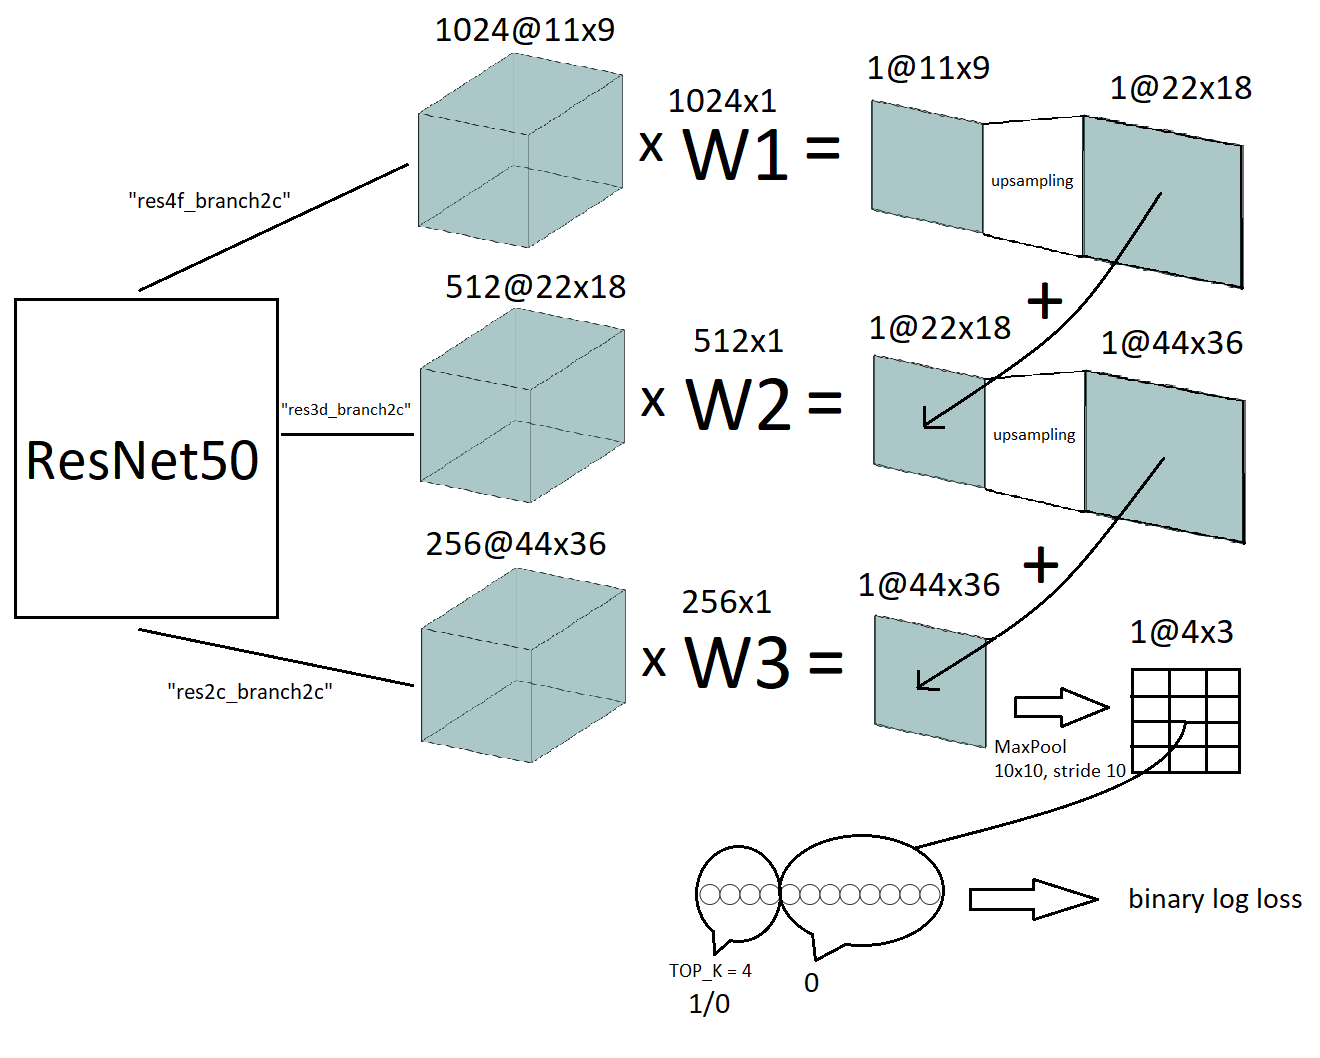
\includegraphics [scale=0.6] {images/schema_total.png}
  \caption{Схема архитектуры} 
  \label{fig:schema_total}  
\end{figure}

В последующих разделах будет обсуждаться подбор параметров системы и параметров обучения, предложенный порядок обучения(\ref{fig:schema_order}), в частности, порядок следования пп.3 и 4, а также будут приведены численные результаты экспериментов с учётом кросс-валидации.



\clearpage